\documentclass{beamer}
\usepackage{pgf-pie}

\begin{document}
	
	\begin{frame}{Bridge Condition Distribution in Germany}
		\centering
		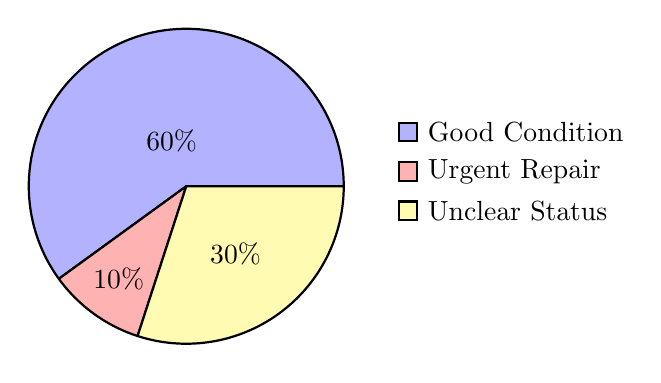
\begin{tikzpicture}
			\pie[
			text=legend,
			sum=100,
			radius=2,
			color={blue!30, red!30, yellow!30}
			]{
				60/Good Condition, 
				10/Urgent Repair, 
				30/Unclear Status
			}
		\end{tikzpicture}
	\end{frame}
	
\end{document}

%\documentclass{beamer}
%\usepackage{tikz}
%
%\begin{document}
%	
%	\begin{frame}{Bridge Conditions in Germany}
%		\centering
%		\begin{tikzpicture}
%			% Draw circles
%			\draw[fill=blue!30, draw=blue] (0,0) circle (2) node[above] {Total Bridges \\ 100\%};
%			\draw[fill=red!30, draw=red] (1.5,0) circle (1.2) node[right] {Urgent Repair \\ 10\%};
%			\draw[fill=yellow!30, draw=yellow] (-1.5,0) circle (1.2) node[left] {Unclear Status \\ 30\%};
%		\end{tikzpicture}
%	\end{frame}
%	
%\end{document}
%
